\documentclass{article}
\usepackage[normalem]{ulem}
\usepackage[utf8]{inputenc}
\usepackage{graphicx}
\usepackage{mathtools}
\usepackage{amssymb}
\usepackage{amsmath}
\usepackage{macros}
\usepackage{color}
\newcommand{\xa}{x-a}
\newcommand{\xan}[1]{(\xa)^{#1}}
\newcommand{\xab}{x^2+ax+b^2}
\newcommand{\xabn}[1]{(\xab)^{#1}}
\newcommand{\intx}[1]{\int^x_a{#1\ dt}}

\begin{document}
\section{\uline{Sats} (integraler och symmetri)}
Antar $f$ integrerbar

\begin{itemize}
  \item Om $f$ är udda, så är $\int_{-a}^a{f(x)\ dx}=0$\\
    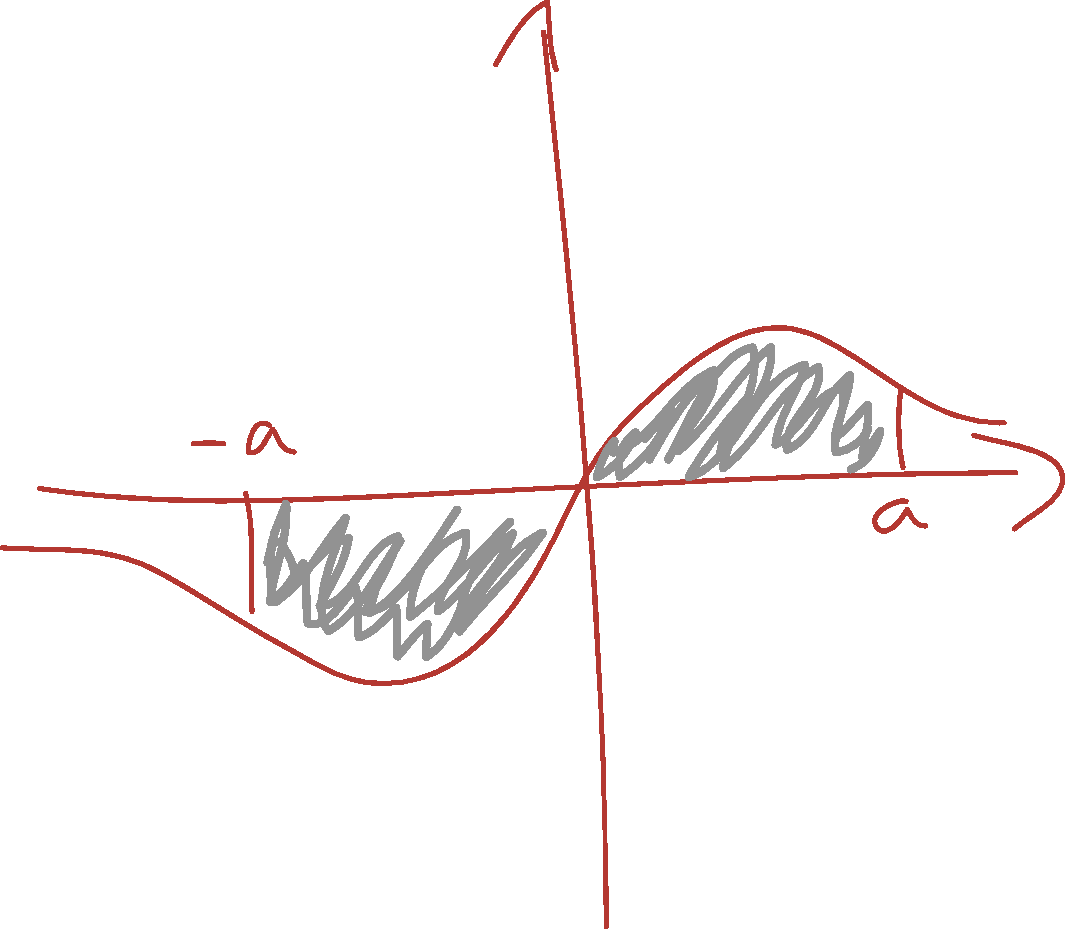
\includegraphics[scale=0.25]{img/img1.pdf}
  \item Om $f$ är jämn, så är $\int_{-a}^a{f(x)\ dx}=2\int_0^a{f(x)\ dx}$\\
    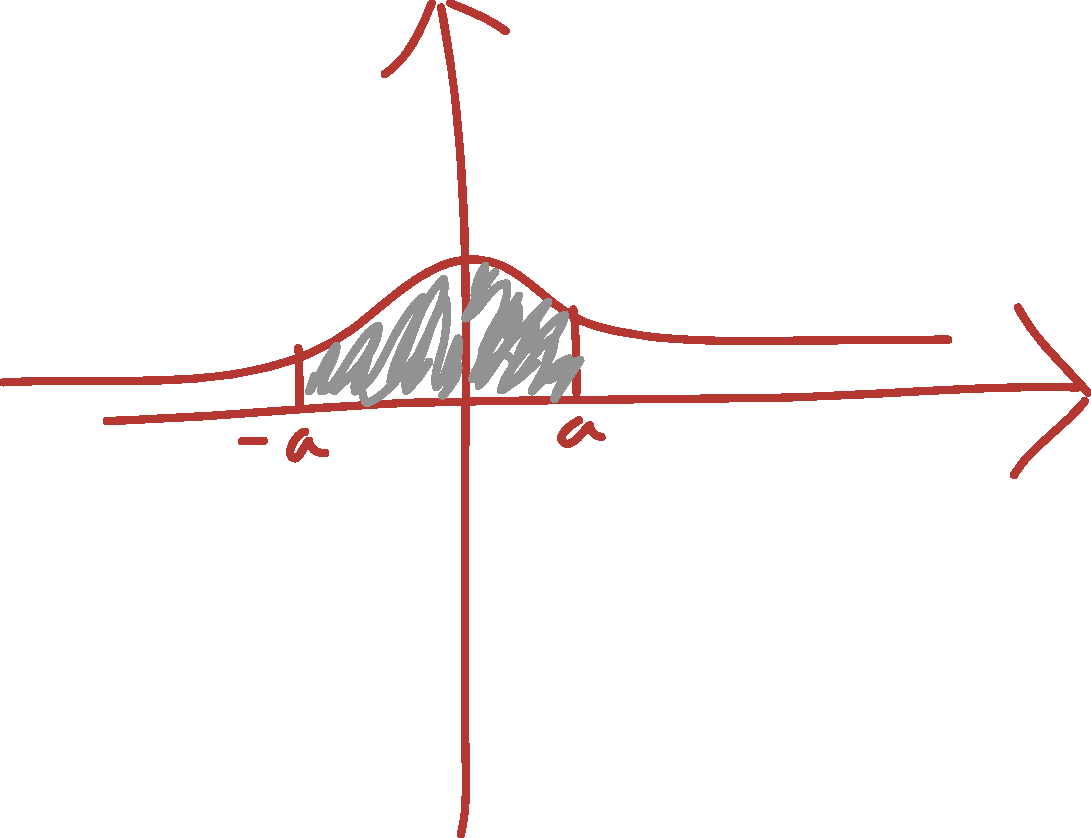
\includegraphics[scale=0.25]{img/img2.pdf}
  \item Om $f$ har period $P$, så är $\int^{a+p}_a{f(x)\ dx}=\int^{b+p}_b{f(x)\ dx}$ för alla a och b.\\
    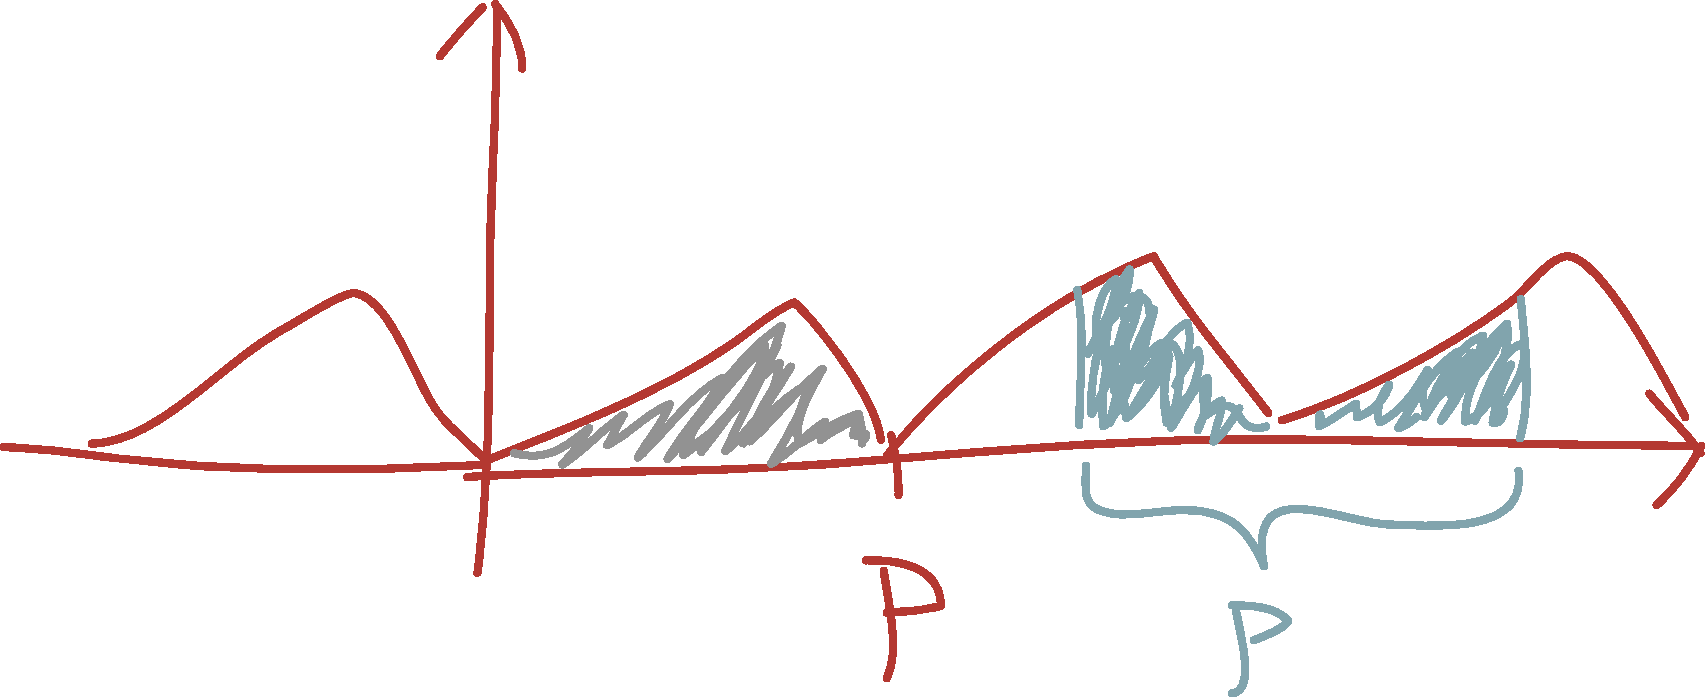
\includegraphics[scale=0.25]{img/img3.pdf}
\end{itemize}

\section{Exempel}
$$ \int^{5\pi \over 8}_{3\pi \over 8}{\cos^3 x\ dx}=\bmat{t=x-\f{\pi}{2}\\x=\f{5 \pi}8 \eq t=\f{\pi}8 \\x=\f{3 \pi}8 \eq t=-\f\pi 8\\dt=dx\\ \cos x = \cos\pa{t+\f\pi 2} = -\sin t}=
\int^{\pi \over 8}_{-\pi \over 8}{\sin^3 t\ dt} = 0 $$

\section{Exempel}
Funktionen $f(x)=\cos^3 x = \f 12 + \f 12 \cos 2x$ har perioden $\pi$

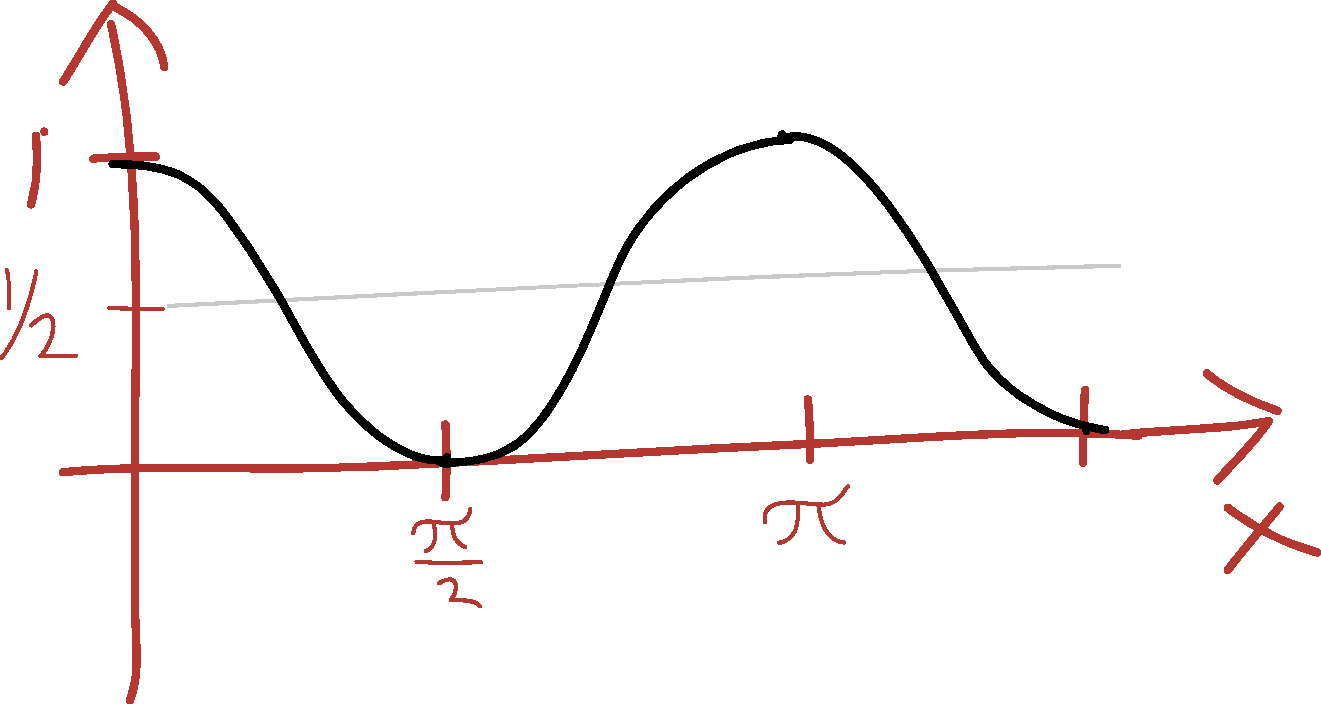
\includegraphics[scale=0.25]{img/img4.pdf}

Integralen av $cos 2x$ över en period är noll.\\
Ifall man integrerar över ett helt antal perioder, dvs om $b-a = (heltal)\pi$, så är alltså
$$ \int^b_a{\cos^2 x\ dx} = \int^b_a{\f 12\ dx}+ \int^b_a{\f 12 \cos 2x\ dx} = \f 12 (b-a) $$

\section{Exempel (Summauppskattning med integraler)}
Vi ska uppskatta hur stor $n! $ är.
Låt $S_n = \ln(n!) = \ln(1\times 2\times 3\times\dots\times n) = \ln 1 + \ln 2 + \ln 3 + \dots + \ln n$

Jämför följande tre figurer:
\begin{enumerate}
  \item
    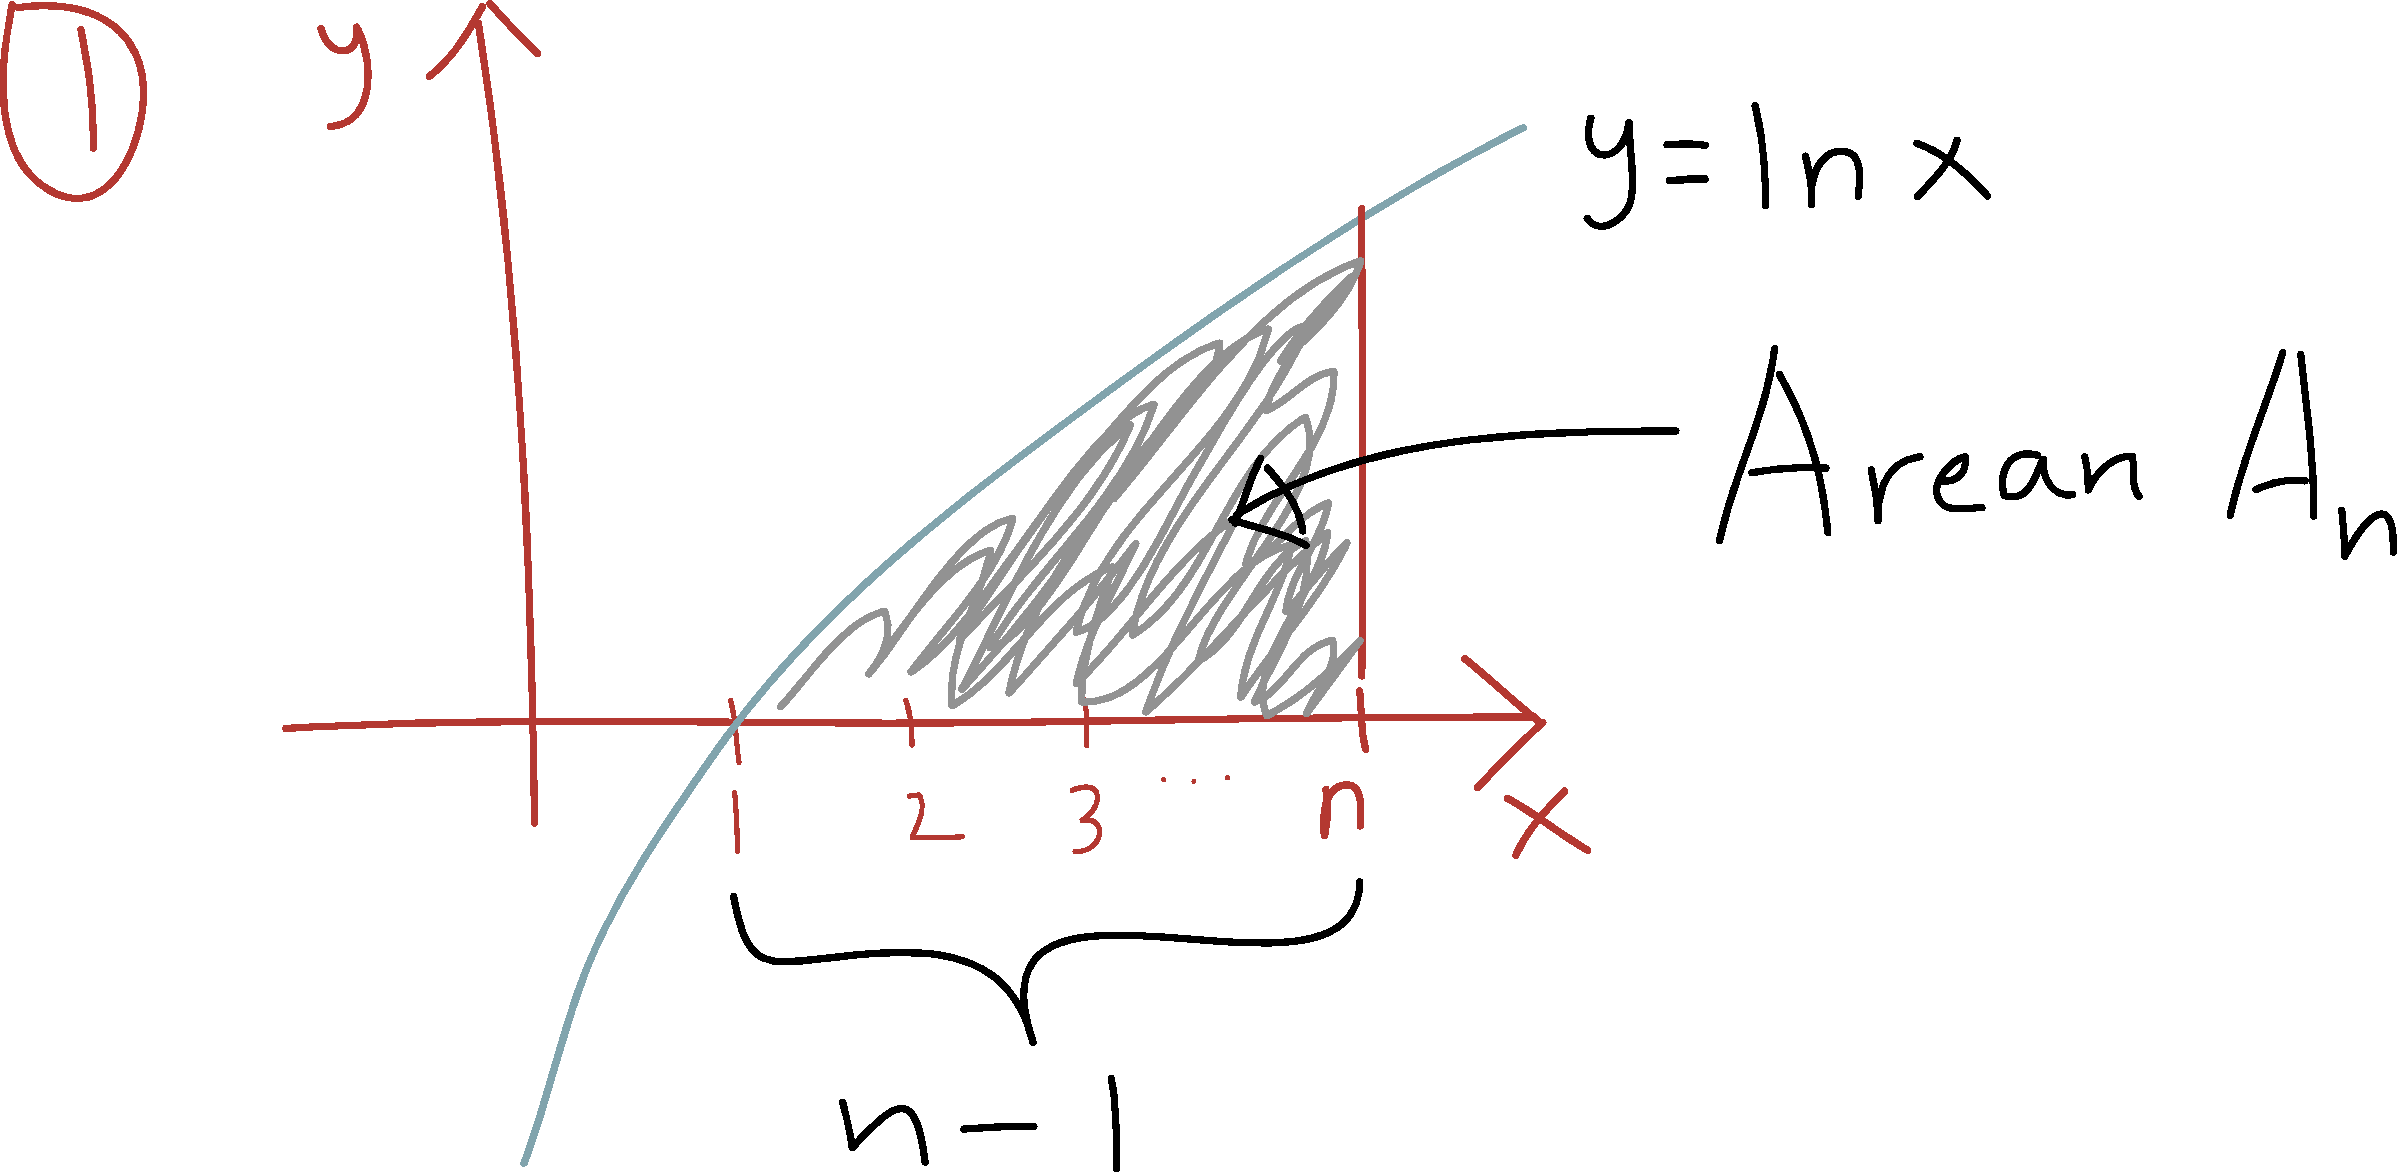
\includegraphics[scale=0.25]{img/img5.pdf}\\
    $$ A_n =\int^n_1{\ln x\ dx} = \bmat{x \ln x - x}^n_1 = (n\ln n - n) - (0-1) = \ln(n^n) + (1-n)$$
  \item
    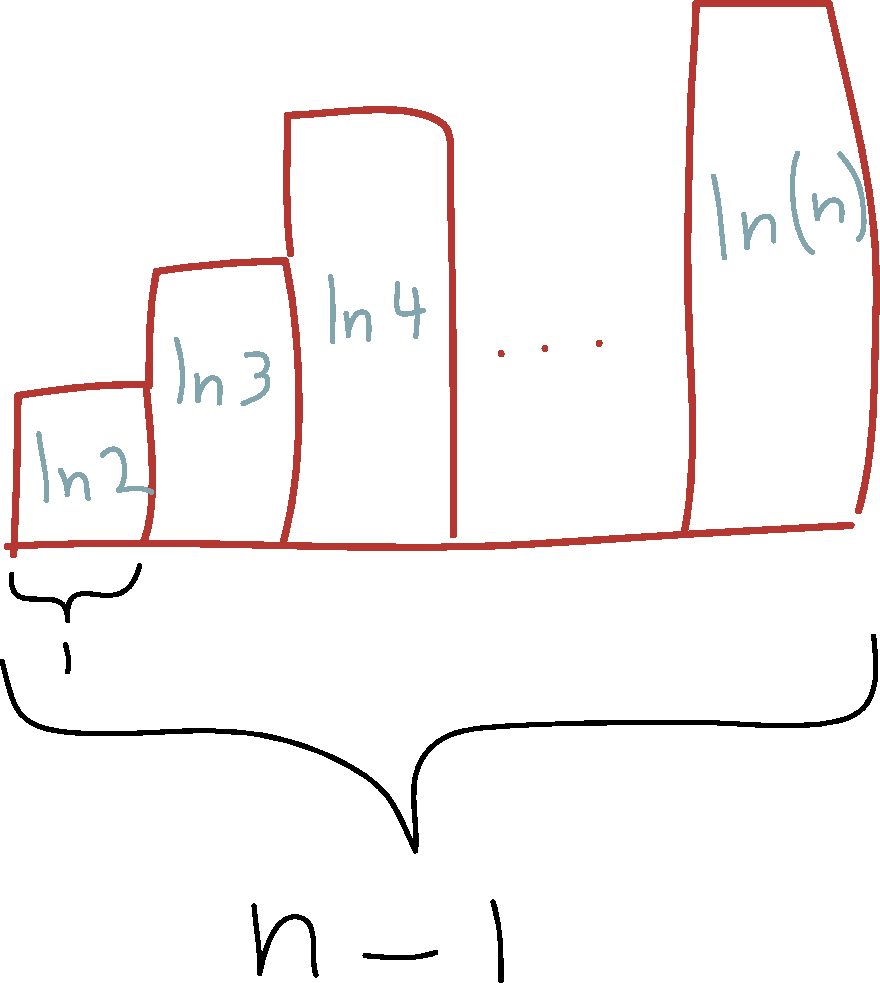
\includegraphics[scale=0.25]{img/img6.pdf}\\
    $$ Area = \ln 2 + \dots + \ln n = S_n $$
  \item
    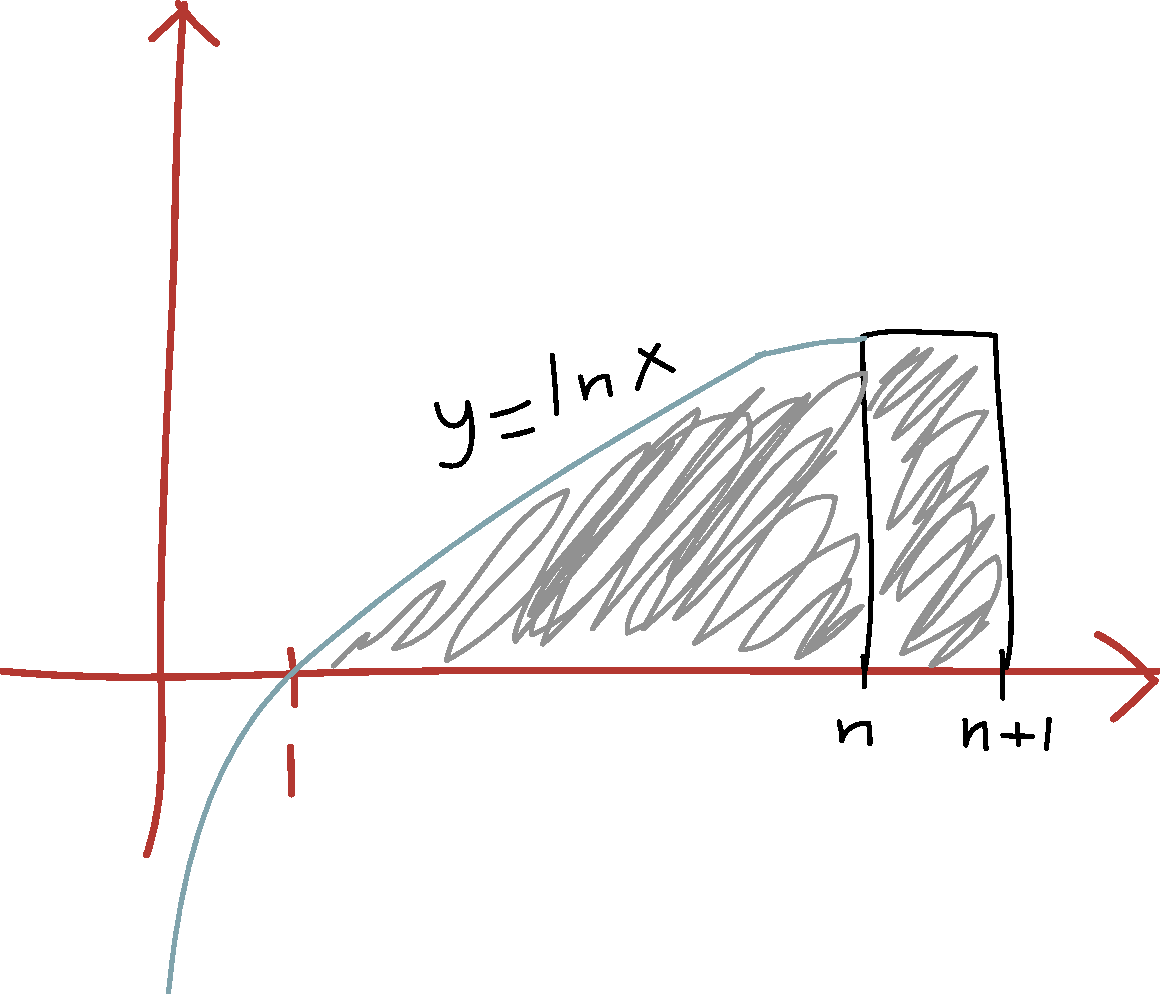
\includegraphics[scale=0.25]{img/img7.pdf}\\
    $$ Area = A_n + \ln n $$
\end{enumerate}

$ (Area 1) < (Area 2) $\\
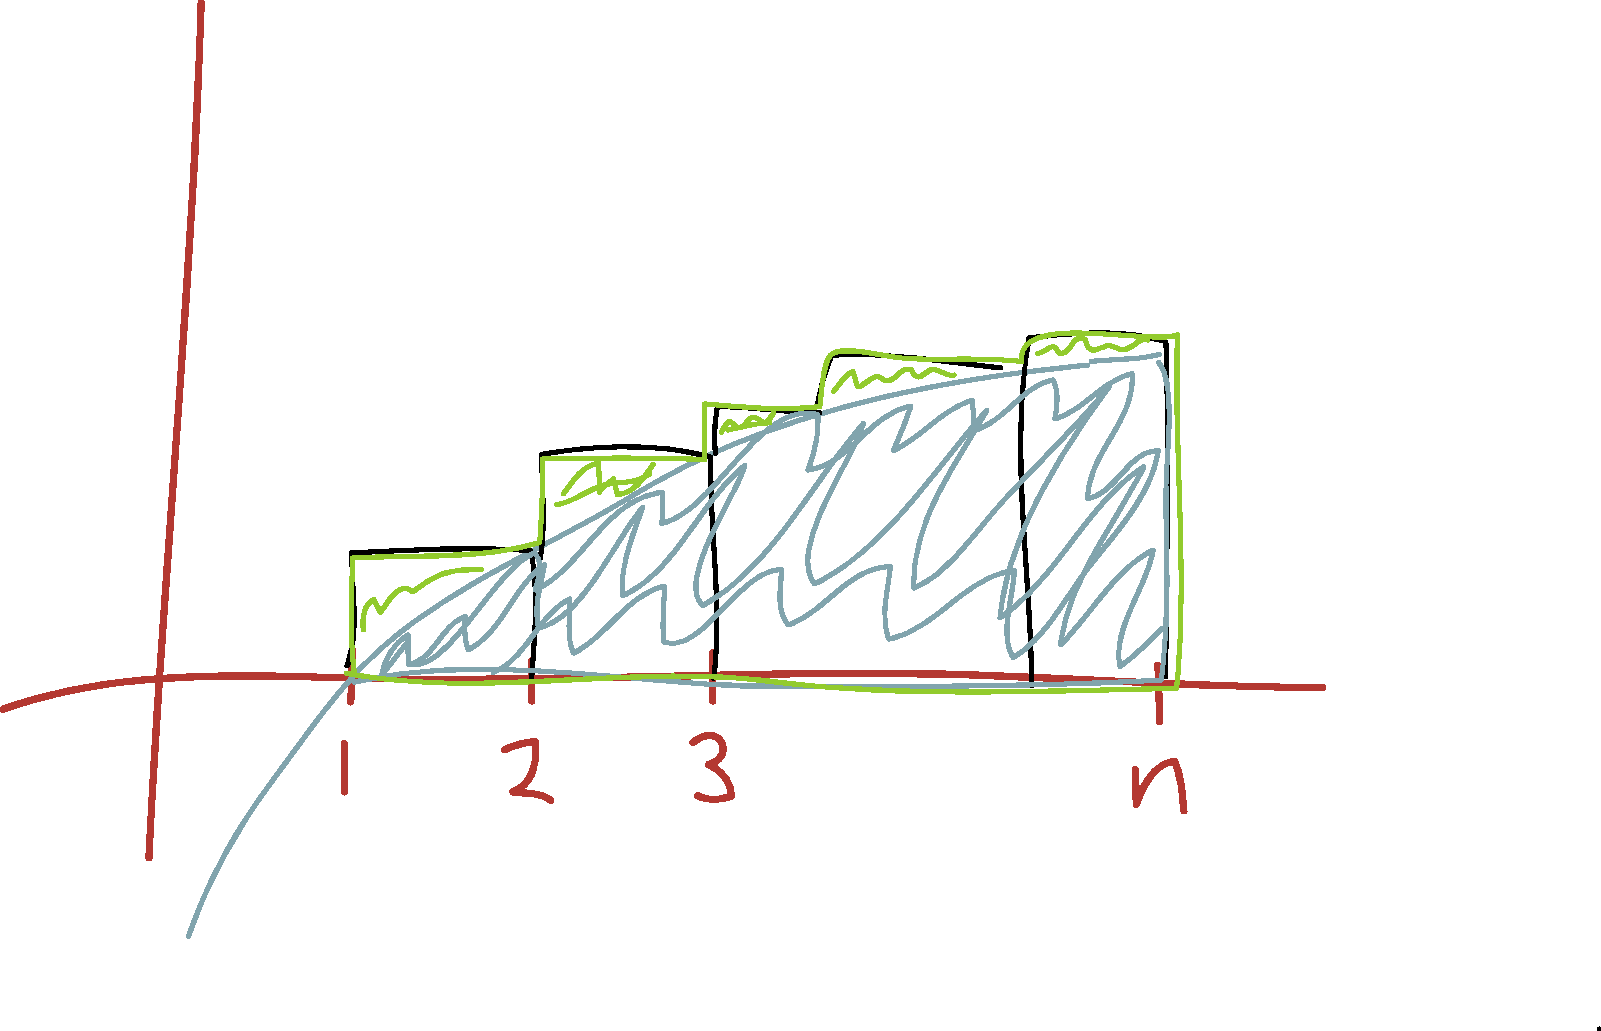
\includegraphics[scale=0.25]{img/img8.pdf}\\

$ (Area 2) < (Area 3) $\\
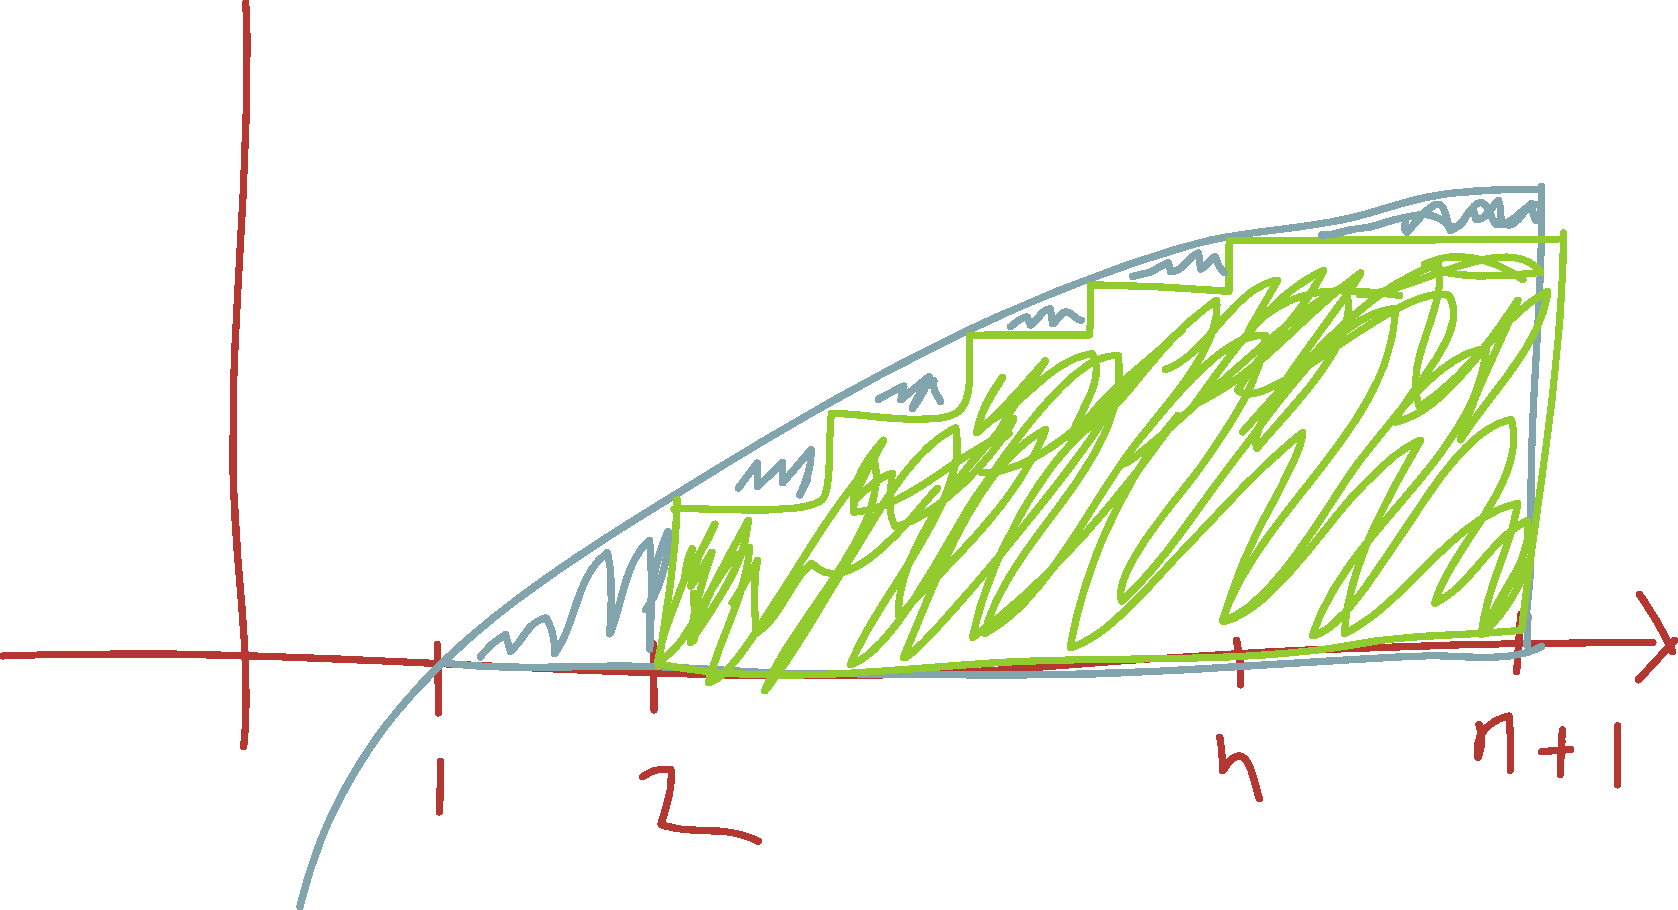
\includegraphics[scale=0.25]{img/img9.pdf}

Alltså:
$$ A_n < S_n < A_n + \ln n $$
($\exp$ är växande)
$$ \im e^{A_n} < e^{S_n} < e^{An+\ln n} $$
$$ \im e^{ln(n^n) + (1-n)} < e^{ln(n!)} < e^{ln(n^n)} + (1-n) + \ln n $$
$$ \im n^n e^{1-n} < n! < n^{n+1} e^{1-n} $$

\section{Generaliserade integraler}
Riemanns def av besämd integral kräver \uline{begränsat} intervall $[a,b]$ och \uline{begränsad} integrand $f(x)$.

\subsection{Definition}
Om $f$ är integrerbar på intervallet $[a,\omega]$ för alla $\omega>a$
Så definierar vi den \uline{generaliserade integralen}
$$ \int^\infty_a{f(x)\ dx}=\lim_{\omega\to\infty} \int^\omega_a{f(x)\ dx} $$
om gränsvärdet existerar ändligt (då sägs integralen vara \uline{konvergent}; annars \uline{divergent}).

\subsection{Exempel}
$$ \int^\omega_1{dx \over x^2} = \bmat{-\f 1x}^\omega_1 = 1-\f 1\omega \to 1, \omega \to \infty $$
så
$$ \int^\infty_1{dx \over x^2} = 1 $$\\

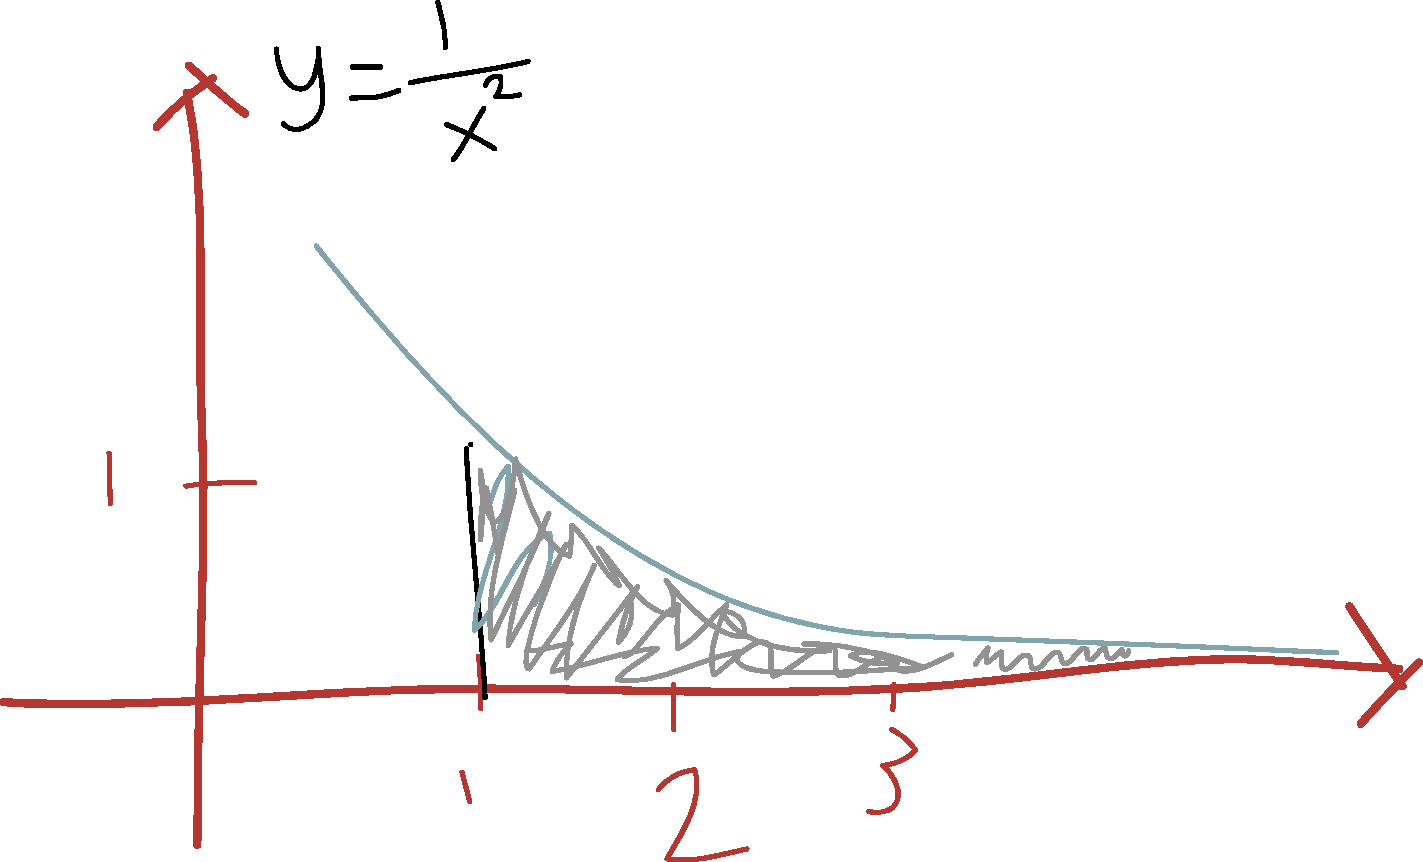
\includegraphics[scale=0.25]{img/img10.pdf}

\subsection{Exempel}
$$ \int^\omega_1{dx \over x} = \ln x \to \infty, \omega \to \infty $$
så $ \int^\infty_1{dx \over x} $ är divergent\\

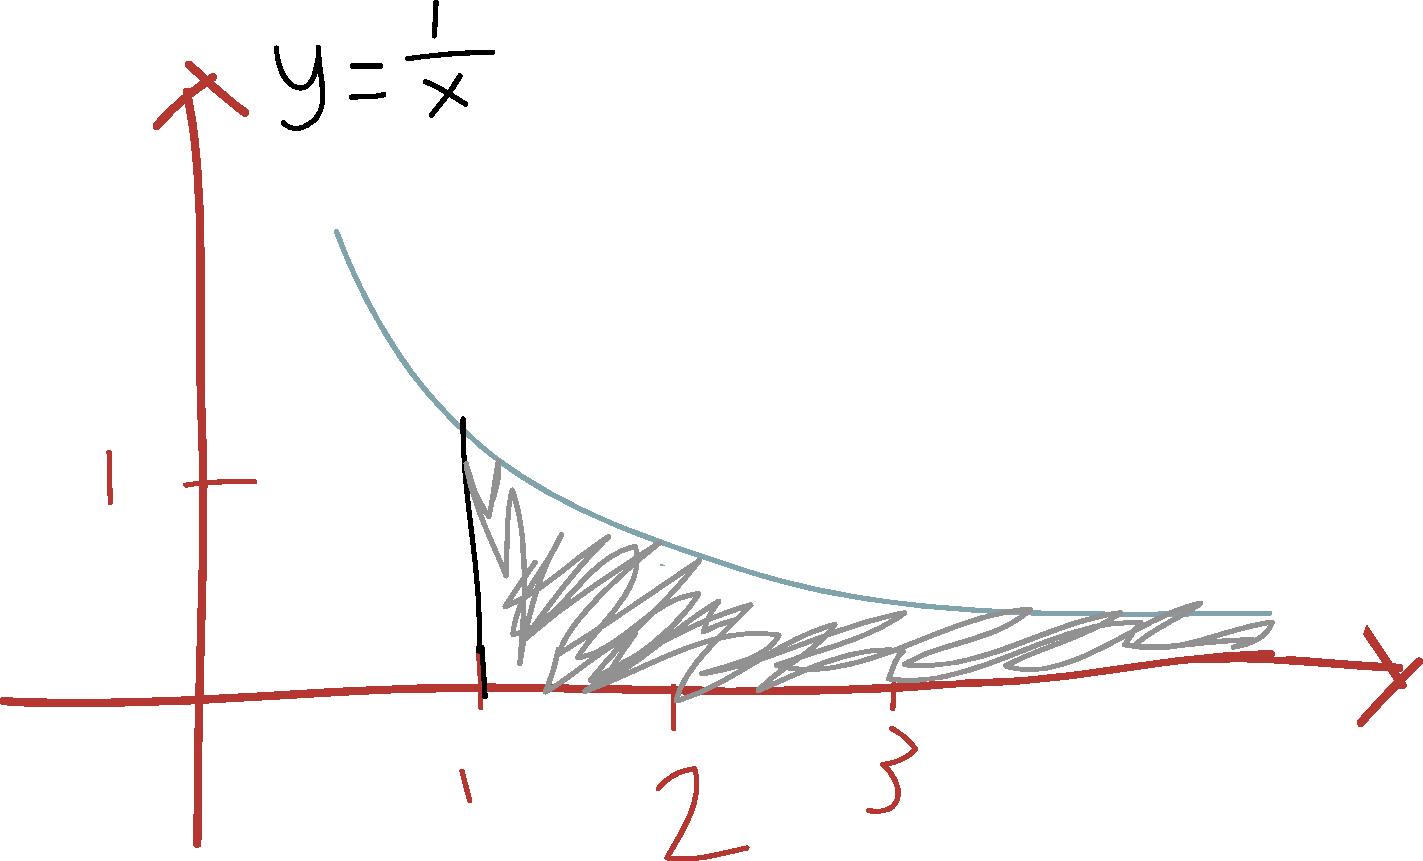
\includegraphics[scale=0.25]{img/img11.pdf}

\subsection{Exempel}
$$ \int^\omega_2{dx \over x^2-1} = \dots = \bmat{\f 12 \pa{\ln\abs{x-1} - \ln\abs{x+1}}}^\omega_2 = $$
$$ \f 12 \pa{\ln\abs{\f{x-1}{x+1}} - \ln\f 13} =$$
$$ \f 12 \pa{\ln\abs{\f{1-\f 1\omega}{1+\f 1\omega}} + \ln 3} \to \f 12 \pa{\ln 1 + \ln 3} = \f{\ln 3}2, \omega \to \infty$$
Alltså
$\int^\infty_2{dx \over x^2-1} = \f{\ln 3}2$

\subsection{Definition}
Antag att $f$ är obegränsad på intervallet $[a,b]$ (eller $]a,b]$) men begränsad och integrerbar på varje delintervall av typen $[c,b]$ där $a<b\le b$\\
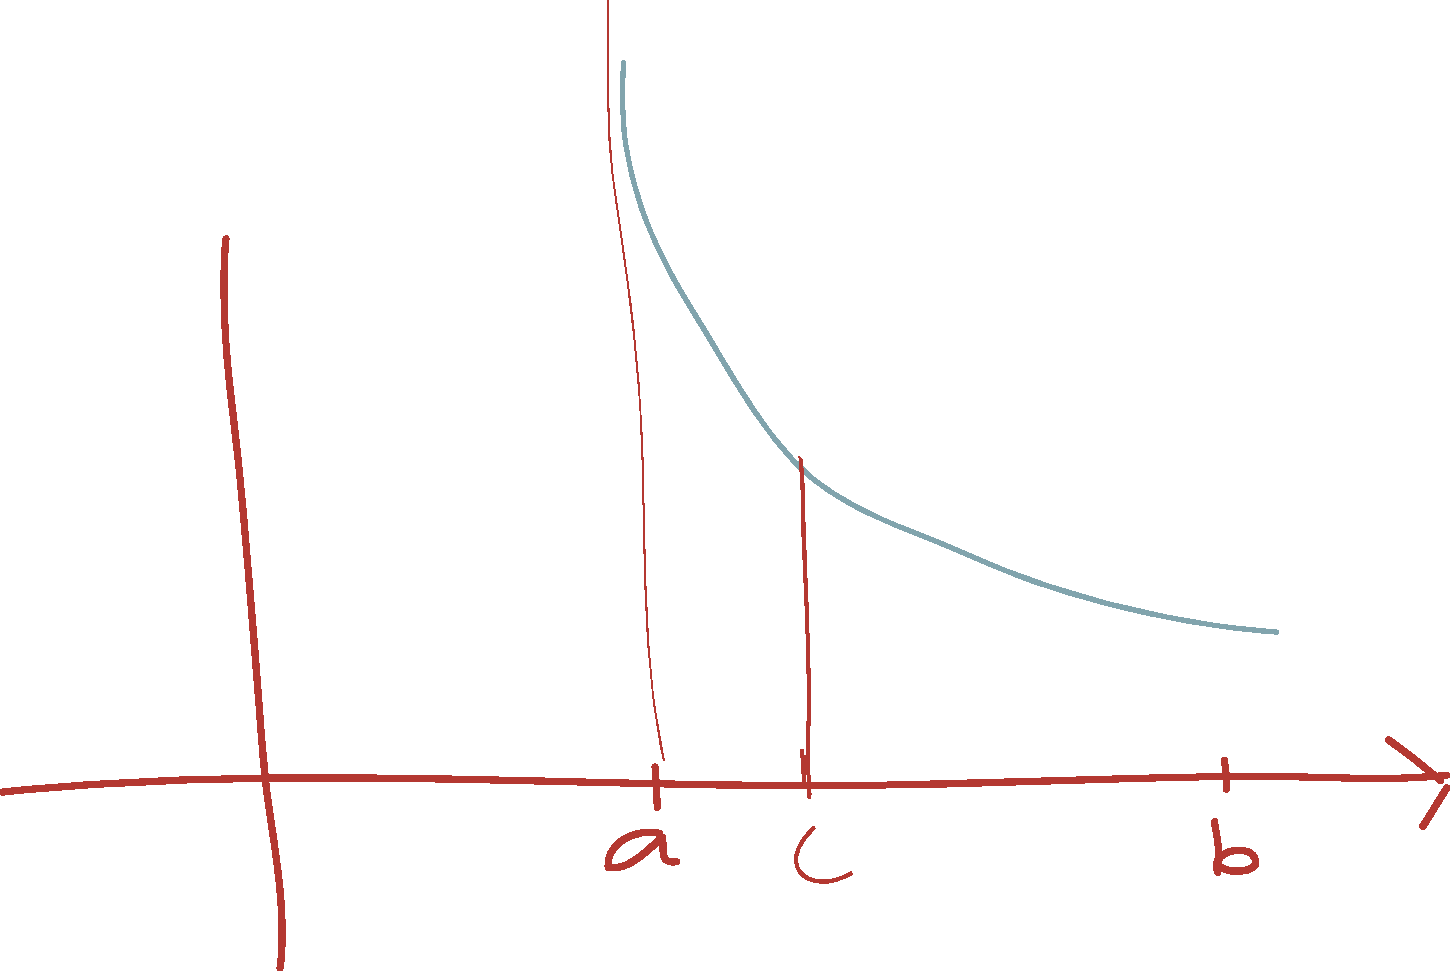
\includegraphics[scale=0.25]{img/img12.pdf}\\
Då sätter vi $\int^b_a{f(x)\ dx} = \lim_{c\to a^+} \int^b_a{f(x)\ dx}$ (om gränsvärde existerar (ändligt))

\subsection{Exempel}
$f(x)=\f 1{\sqrt{x}}$ är obegränsat på intervallet $]0,1]$\\
För $0<c\le 1$ är $\int^1_c{dx \over \sqrt{x}} = \bmat{2\sqrt{x}}^1_c = 2-2\sqrt{c} \to 2, c\to 0^+$\\
Så $\int_0^1{\f {dx}{\sqrt{x}}} = 2$\\
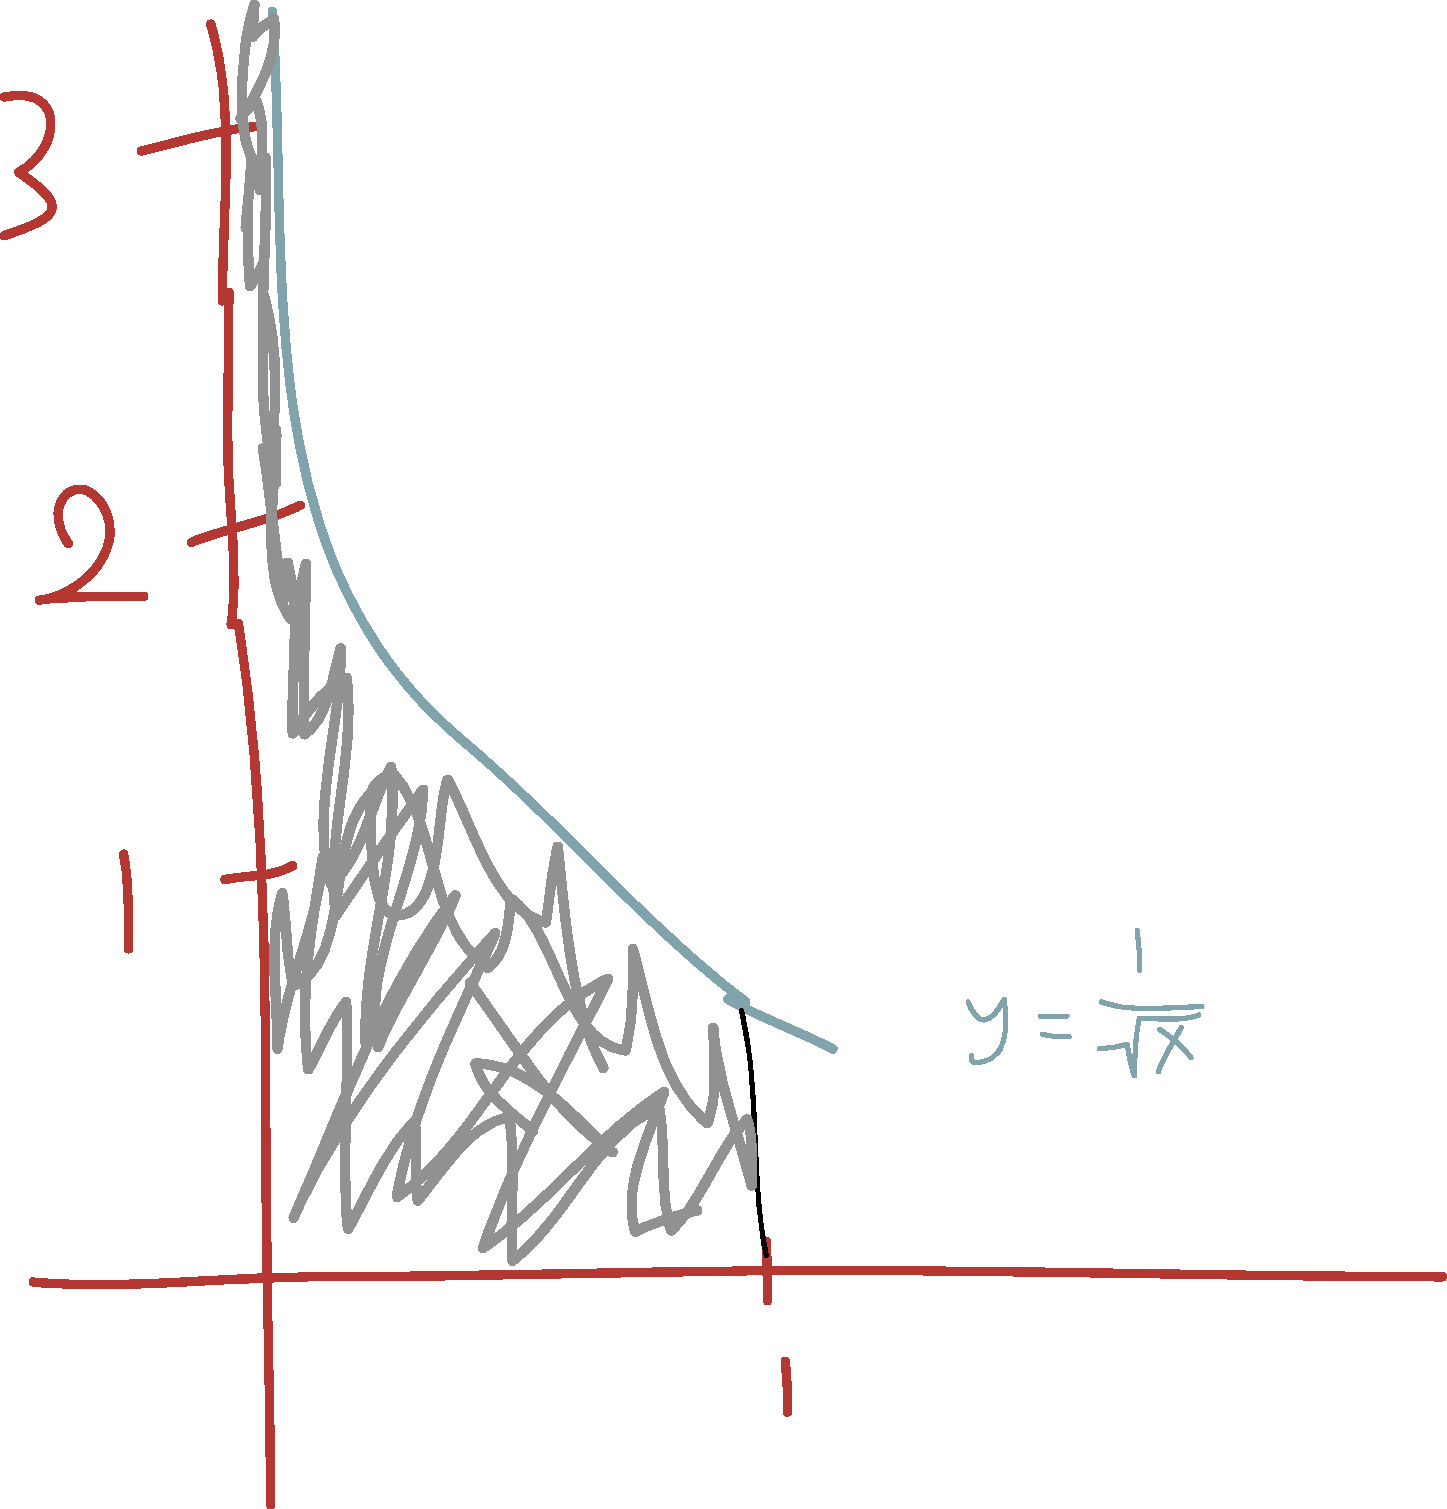
\includegraphics[scale=0.25]{img/img13.pdf}

\subsection{}
Om integralen är generaliserad på flera sätt måste man dela upp den i delar som var och en är generaliserade på vara ett sätt.

\subsection{Exempel}
$$ \int^\infty_0{dx \over x^2} = \int^1_0{dx \over x^2} + \int^\infty_1{dx \over x^2} $$
är \uline{divergent}.

\subsection{Exempel}
$$ \int^1_{-1}{dx \over x} = \int^0_{-1}{dx \over x} + \int^1_0{dx \over x} $$
är \uline{divergent}.\\
Inte såhär:

$$ \int^1_{-1}{dx \over x} = (fel!) = \bmat{\ln\abs{x}}^1_{-1} = \ln 1 - \ln 1 = 0 $$

\end{document}
